\documentclass{standalone}

\usepackage{xcolor}

\definecolor{myblue}{HTML}{377EB8}
\definecolor{myred}{HTML}{E41A1C}

\usepackage{tikz}
\usepackage{pgfplots}
\pgfplotsset{compat=newest}

\usepackage{lmodern}
\SetSymbolFont{letters}{bold}{OML}{cmbr}{bx}{it}
\renewcommand{\familydefault}{\sfdefault}

\usepackage{sansmathfonts}

\begin{document}
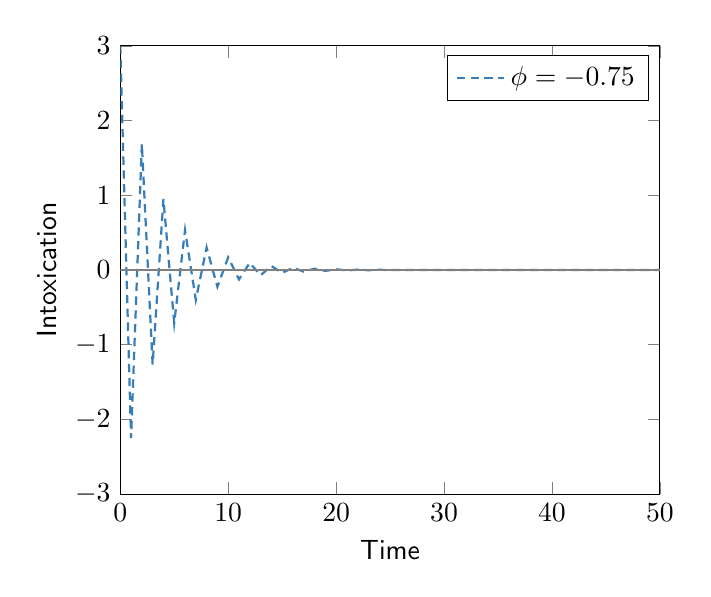
\begin{tikzpicture}
	\begin{axis}[
			xlabel={Time},
			ylabel={Intoxication},
			xmin=0, xmax=50,
			ymin=-3, ymax=3,
			xtick={0,10,20,30,40,50},
			ytick={-3,-2,-1,0,1,2,3},
			grid style=dashed,
		]		
		\addplot[
			color=myblue,
            thick,
            densely dashed
		]
		coordinates {
			(0, 3)
			(1, -2.25)
			(2, 1.6875)
			(3, -1.265625)
			(4, 0.94921875)
			(5, -0.7119140625)
			(6, 0.533935546875)
			(7, -0.40045166015625)
			(8, 0.300338745117188)
			(9, -0.225254058837891)
			(10, 0.168940544128418)
			(11, -0.126705408096313)
			(12, 0.095029056072235)
			(13, -0.071271792054176)
			(14, 0.053453844040632)
			(15, -0.040090383030474)
			(16, 0.030067787272856)
			(17, -0.022550840454642)
			(18, 0.016913130340981)
			(19, -0.012684847755736)
			(20, 0.009513635816802)
			(21, -0.007135226862601)
			(22, 0.005351420146951)
			(23, -0.004013565110213)
			(24, 0.00301017383266)
			(25, -0.002257630374495)
			(26, 0.001693222780871)
			(27, -0.001269917085653)
			(28, 0.00095243781424)
			(29, -0.00071432836068)
			(30, 0.00053574627051)
			(31, -0.000401809702883)
			(32, 0.000301357277162)
			(33, -0.000226017957871)
			(34, 0.000169513468404)
			(35, -0.000127135101303)
			(36, 9.54E-05)
			(37, -7.15E-05)
			(38, 5.36E-05)
			(39, -4.02E-05)
			(40, 3.02E-05)
			(41, -2.26E-05)
			(42, 1.70E-05)
			(43, -1.27E-05)
			(44, 9.55E-06)
			(45, -7.16E-06)
			(46, 5.37E-06)
			(47, -4.03E-06)
			(48, 3.02E-06)
			(49, -2.27E-06)
			(50, 1.70E-06)
			(51, -1.27E-06)
			(52, 9.56E-07)
			(53, -7.17E-07)
			(54, 5.38E-07)
			(55, -4.03E-07)
			(56, 3.02E-07)
			(57, -2.27E-07)
			(58, 1.70E-07)
			(59, -1.28E-07)
			(60, 9.57E-08)
			(61, -7.18E-08)
			(62, 5.38E-08)
			(63, -4.04E-08)
			(64, 3.03E-08)
			(65, -2.27E-08)
			(66, 1.70E-08)
			(67, -1.28E-08)
			(68, 9.58E-09)
			(69, -7.18E-09)
			(70, 5.39E-09)
			(71, -4.04E-09)
			(72, 3.03E-09)
			(73, -2.27E-09)
			(74, 1.70E-09)
			(75, -1.28E-09)
			(76, 9.59E-10)
			(77, -7.19E-10)
			(78, 5.39E-10)
			(79, -4.05E-10)
			(80, 3.03E-10)
			(81, -2.28E-10)
			(82, 1.71E-10)
			(83, -1.28E-10)
			(84, 9.60E-11)
			(85, -7.20E-11)
			(86, 5.40E-11)
			(87, -4.05E-11)
			(88, 3.04E-11)
			(89, -2.28E-11)
			(90, 1.71E-11)
			(91, -1.28E-11)
			(92, 9.61E-12)
			(93, -7.21E-12)
			(94, 5.41E-12)
			(95, -4.05E-12)
			(96, 3.04E-12)
			(97, -2.28E-12)
			(98, 1.71E-12)
			(99, -1.28E-12)
		};
		\draw[gray] (0,0) -- (100,0);
		\legend{$\phi = -0.75$}
	\end{axis}
\end{tikzpicture}
\end{document}

% time <- 100
% phi <- 0.75
% y <- rep(x = NA, times = time)
% y[1] <- +3
% for (i in 2:time) {
%   y[i] <- phi * y[i - 1]
% }
% plot(y, type = "l")
% y
